\section{Type-Matcher Rating basierte Heuristiken}
Wie die �berschrift bereits andeutet, werden die Type-Matcher mit einem Rating versehen. Das Rating wird durch einen numerischen Wert dargestellt. Auf dieser Basis werden zwei Kategorien von Type-Matcher Ratings unterschieden:
\myparagraph{Qualitatives Type-Matcher Rating}
Das qualitative Type-Matcher Rating beschreibt den Grad der strukturellen �bereinstimmung des Source- und des Target-Typen. Daf�r wird jeder Type-Matcher mit einem Basiswert versehen. Die konkreten Basiswerte sind im Abschnitt Evaluation beschrieben. Dieser Basiswert wird beim Erzeugen der Typ-Konvertierungsvarianten an die methodendelegationsrelevanten Informationen geh�ngt, sodass zu jeder Methode, zu der eine Methoden-Konvertierungsvariante existiert, auch ein Wert bzgl. des qualitatives Type-Matcher Ratings zur Verf�gung steht.\\\\
Der konkrete Wert f�r das qualitative Type-Matcher-Rating ermittelt sich grundlegend, wie bereits erw�hnt, anhand eines Basiswertes. Sofern ein Type-Matcher jedoch wiederum eine �bereinstimmung verwendeter Typen fordert, um die konkreten methodendelegationsrelevanten Informationen zu erzeugen (WrappedTypeMatcher und StructuralTypeMatcher), ergibt sich der Wert des Type-Matcher-Ratings aus einer Akkumulation der Basiswerte aller verwendeten Type-Matcher.\\\\
Damit ist das qualitative Type-Matcher Rating von folgenden Faktoren abh�ngig:
\begin{enumerate}
\item Die Wahl des Basiswertes der einzelnen Type-Matcher
\item Das Akkumulationsverfahren f�r das Type-Matcher Rating einer Typ-Konvertierungsvariante
\item Das Akkumulationsverfahren f�r das Type-Matcher Rating einer Methoden-Konvertierungsvariante
\end{enumerate}
Alle drei Punkt werden bei der Evaluierung dieser Heuristik untersucht.
\myparagraph{Quantitatives Type-Matcher Rating}
Das quantitative Type-Matcher Rating beschreibt, zu wie vielen der erwarteten Methoden in der erzeugten Typ-Konvertierungsvariante methodendelegationsrelevante Informationen vorliegen. So stellt das quantitative Type-Matcher Rating also einen Prozentsatz dar.\\\\
Im Folgenden werden zwei Heuristiken vorgestellt, die auf den oben genannten Type-Matcher Ratings basieren.
\subsection{TMR\_Quant: Beachtung des quantitativen Type-Matcher Ratings}\label{tmr_quant}
\myparagraph{Szenario}
\abbref{tmr_quantScen} zeigt ein Szenario, in dem ein erwartetes Interface IExpect mit zwei Methoden deklariert wurde. Auf der rechten Seite sind die beiden angebotenen Interfaces abgebildet (IOfferedA und IOfferedB), die laut den oben genannten Type-Matchern zu dem erwarteten Interface passen. Weiterhin soll in diesem Szenario davon ausgegangen werden, dass eine passende ben�tigte Komponente (Proxy) nur aufbauend auf den Methoden-Konvertierungsvarianten erzeugt werden kann, die auf der Basis des angebotenen Interfaces IOfferedB erzeugt werden k�nnen.
\myBigFigure{Scen_TMR_Quant}{Szenario f�r TMR\_Quant}{tmr_quantScen}
\noindent
%Es wird davon ausgegangen, dass eine angebotene Komponente, deren Schnittstelle strukturell mit der erwarteten Schnittstelle �bereinstimmt und dabei zu jeder erwarteten Methode eine passende Methode anbietet, eher die semantischen Erwartungen erf�llt, als eine Kombination aus mehreren angebotenen Komponenten. 
\myparagraph{Exploration ohne Heuristik}
Der Explorationsalgorithmus w�rde die passende ben�tigte Komponente im ersten Durchlauf finden. Allerdings w�rde auch die Typ-Konvertierungsvariante f�r IOfferedA im schlimmsten Fall innerhalb des ersten Durchlaufs analysiert werden. Die Kombinationen von Typ-Konvertierungsvarianten der beiden angebotenen Interfaces, die im ersten Durchlauf des Explorationsalgorithmus erzeugt werden, sind \abbref{tmr_quant_tkvkombi} zu entnehmen. Darauf aufbauend, w�rde aus diesen Kombinationen von Typ-Konvertierungsvarianten die Kombinationen von Methoden-Konvertiertungsvarianten erzeugt werden, welche \abbref{tmr_quant_mkvkombi} zu entnehmen sind.


\begin{figure}[H]
\begin{minipage}[b]{.38\linewidth}
  \centering
  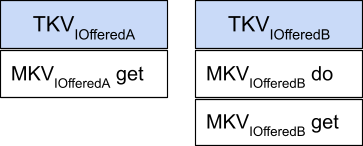
\includegraphics[width=\linewidth]{tmr_quant_tkvkombis}
  \captionof{figure}{Typ-Konvertierungsvarianten dem Szenario zu TMR\_Quant}
  \label{abb:tmr_quant_tkvkombi}

\end{minipage}%
\hspace{.04\linewidth}% Abstand zwischen Bilder
\begin{minipage}[b]{.58\linewidth}


  \centering
  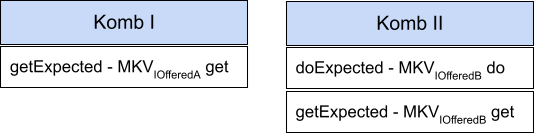
\includegraphics[width=\linewidth]{tmr_quant_mkvkombis}
  \captionof{figure}{Methoden-Konvertierungsvarianten dem Szenario zu TMR\_Quant}
  \label{abb:tmr_quant_mkvkombi}

\end{minipage}
\end{figure}
\myparagraph{Ableitung der Heuristik}
Hierbei f�llt auf, dass das Erzeugen der Methoden-Konvertierungsvarianten f�r IOfferedA unn�tig war, weil nur f�r eine der erwarteten Methoden eine Methoden-Konvertierungsvariante erzeugt werden konnte. Dies kann durch die Beachtung des quantitativen Type-Matcher Ratings im ersten Durchlauf des Explorationsalgorithmus verhindert werden.\\\\
Hierzu werden im Schritt 2 der 2. Stufe des Explorationsalgorithmus (siehe \ref{sem_eval_step2}) nur die Typ-Konvertierungsvarianten als Ergebnis ermittelt, die ein quantitatives Type-Matcher Rating von 100\% aufweisen. Damit wird bezogen auf das Szeanrio nur die Typ-Konvertierungsvariante des angebotenen Interfaces IOfferedB weiter analysiert.
\subsection{TMR\_Qual: Beachtung des qualitativen Type-Matcher Ratings}\label{tmr_qual}
\myparagraph{Szenario}
\abbref{tmr_qualScen} zeigt ein Szenario, in dem ein erwartetes Interface IExpect mit einer Methode deklariert wurde. Die Deklaration erfolgte unter der Verwendung bestehender allgemeiner Typen innerhalb des gesamten Systems, die in dem unteren Bereich der Abbildung dargestellt sind. Dabei gibt es zwei Typen, die in einer Vererbungsbeziehung stehen (Common und Specific), und einen Wrapper-Typen, der ein Attribut vom Typ Common enth�lt. Zus�tzlich sind auf der rechten Seite die angebotenen Interfaces abgebildet (IOfferedA und IOfferedB), die laut den oben genannten Type-Matchern zu dem erwarteten Interface passen. Auch diese verwenden die allgemeinen Typen. F�r dieses Szenario ist davon auszugehen, dass eine passende ben�tigte Komponente (Proxy) nur aufbauend auf den Methoden-Konvertierungsvarianten erzeugt werden kann, die auf der Basis des angebotenen Interfaces IOfferedB erzeugt werden k�nnen.

\myBigFigure{Scen_TMR_Qual}{Szenario f�r TMR\_Qual}{tmr_qualScen}

\myparagraph{Exploration ohne Heuristik}
Der Explorationsalgorithmus w�rde die passende ben�tigte Komponente im ersten Durchlauf finden. Hierbei werden zuerst die Typ-Konvertierungsvarianten der beiden angebotenen Interfaces erzeugt, welche \abbref{tmr_qual_tkvkombi} zu entnehmen sind. \abbref{tmr_qual_mkvkombi} zeigt die im darauffolgenden Schritt des Explorationsalgorithmus (siehe \ref{sem_eval_step3}) erzeugten Kombinationen von Methoden-Konvertierungsvarianten. Zu erkennen ist, dass auch die Kombinationen von Methoden-Konvertierungsvarainten von IOfferedA erzeugt wurden und demnach im schlimmsten Fall auch weiter analysiert werden.

\begin{figure}[H]
\begin{minipage}[b]{.38\linewidth}
  \centering
  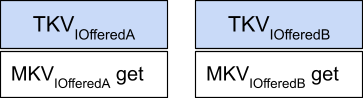
\includegraphics[width=\linewidth]{tmr_qual_tkvkombis}
  \captionof{figure}{Typ-Konvertierungsvarianten dem Szenario zu TMR\_Qual}
  \label{abb:tmr_qual_tkvkombi}

\end{minipage}%
\hspace{.04\linewidth}% Abstand zwischen Bilder
\begin{minipage}[b]{.58\linewidth}


  \centering
  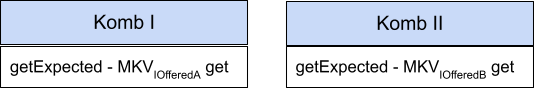
\includegraphics[width=\linewidth]{tmr_qual_mkvkombis}
  \captionof{figure}{Methoden-Konvertierungsvarianten dem Szenario zu TMR\_Qual}
  \label{abb:tmr_qual_mkvkombi}

\end{minipage}
\end{figure}



\myparagraph{Ableitung der Heuristik}
Bei der Betrachtung der Methode, die von der nachfragenden Komponente erwartet und von den angebotenen Komponenten B bereitgestellt wird, f�llt auf, dass die Typen des Parameter und der R�ckgabewerte der jeweiligen Methoden in einer Vererbungsbeziehung stehen. Dadurch ist eine Delegation der Form $\delegate{\text{IExpect}.\text{getExpected}}{\text{IOfferedB}.\text{get}}$ aufgrund des liskovschen Substitutionsprinzip ohne weitere Konvertierung der Parameter- und R�ckgabe-Typen m�glich. Eine Delegation der Methoden aus IExpect an IOfferedA ist hingegen weitaus komplizierter (siehe \ref{wrappedTypeMatcher}).
In Bezug auf das oben beschrieben Type-Matcher Rating bedeutet das, dass das qualitative Type-Matcher Rating der Typ-Konvertierungsvariante von IOfferedB geringer ist, als das der Typ-Konvertierungsvariante von IOfferedA.\\\\
F�r die Heuristik TMR\_Qual kann demnach abgeleitet werden, dass die Kombinationen von Methoden-Konvertierungsvarianten in Schritt 3 der 2. Stufe des Explorationsalgorithmus  (siehe \ref{sem_eval_step3}) zuerst aus denjenigen Kombinationen von Typ-Konvertierungsvarianten mit den niedrigsten qualitativen Type-Matcher Rating erzeugt und analysiert werden sollten.

